\begin{figure}
	\centering%
	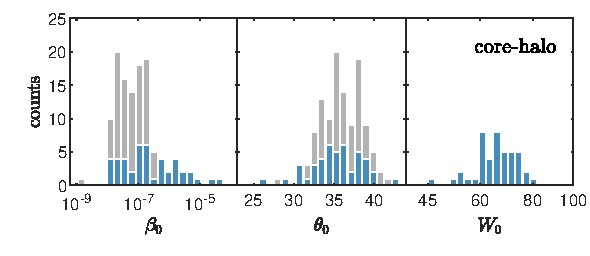
\includegraphics[width=\hsize]{\ROOTPATH/CoreHalo.pdf}
	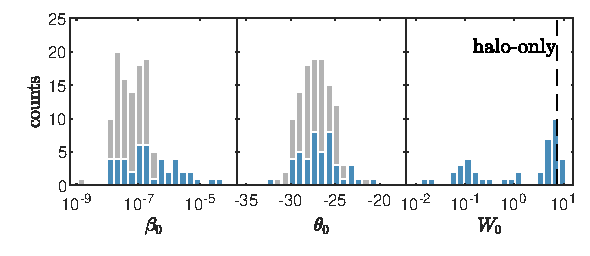
\includegraphics[width=\hsize]{\ROOTPATH/HaloOnly.pdf}
	\caption{Distribution of the best-fit parameters for the fermionic model with a \textit{core-halo} (top) and fully diluted (bottom). The blue bars represent the sub-sample of non-isothermal solutions (44 galaxies) with $W_p \lesssim 10$ (top) and $W_0 \lesssim 10$ (bottom), respectively, while the gray bars include the full sample (120 galaxies). Note that the values at plateau of the core-halo solutions (i.e. $\beta_p$, $\theta_p$, $W_p$) can be identified with the values at the center of the halo-only solutions (i.e. $\beta_0$, $\theta_0$, $W_0$). In the case of halo-only solutions (bottom) the dashed line represents the stability change where fermionic DM halos become unstable for $W_p\equiv W_0 \gtrsim 7.45$. \citep{2015PhRvD..91f3531C}}%
	\label{fig:parameter-distribution:mepp}%
\end{figure}
% For the central cutoff only the sub-sample is shown where best-fits allow to constrain $W_0$